\documentclass[a4paper,11pt]{article}
\usepackage[utf8]{inputenc}
\usepackage[T1]{fontenc}
\usepackage[english]{babel}
\usepackage{graphicx}
\usepackage{hyperref}
\usepackage{amsmath}
\usepackage{geometry}
\geometry{margin=2.5cm}

\title{\textbf{Interactive 3D Melody Generator using Babylon.js and Havok Physics}}
\author{Ismail El Amrani \\ Master 1 Computer Science \\ Universit\'e C\^ote d'Azur}
\date{February -- May 2025}

\begin{document}

\begin{titlepage}
    \centering
    \vspace*{2cm}
    
\includegraphics[width=0.5\textwidth]{logo-Unica.png}\\[2cm]
    \textbf{\Large Travail d'\'Etude et de Recherche}\\[0.5cm]
    \textbf{\Large M1 Informatique}\\[1.5cm]
    \rule{\linewidth}{0.5mm} \\[0.4cm]
    {\huge \bfseries Design and Implementation of a Note Generator for Interactive 3D Musical Experiences\\[0.4cm]}
    \rule{\linewidth}{0.5mm} \\[1.5cm]
    \begin{minipage}[t]{0.4\textwidth}
        \begin{flushleft} \large
        \textbf{Author:} \\
        Mr. Ismail El Amrani
        \end{flushleft}
    \end{minipage}%
    \hfill
    \begin{minipage}[t]{0.4\textwidth}
        \begin{flushright} \large
        \textbf{Student ID:} \\
        22411360
        \end{flushright}
    \end{minipage} \\[1.5cm]
    \textbf{Supervisor:} Mr. Michel BUFFA \\[0.5cm]
    \textbf{Host Laboratory:} I3S Laboratory \\[0.5cm]
    \textbf{Recipients:} Michel BUFFA, Ramon Aparicio, Luc Hogie \\[0.5cm]
    \textbf{Period:} February 2025 -- May 2025
    \vfill
\end{titlepage}

\begin{abstract}
This report presents the design and implementation of an interactive melody generator based on physical interactions in a 3D environment. Using Babylon.js for rendering, Havok for physics simulation, and a WAM synthesizer for real-time sound generation, the project allows the generation of harmonious musical notes from object collisions. The goal is to create an immersive, interactive, and musical experience.
\end{abstract}

\tableofcontents
\newpage

\section{Introduction}
\subsection{Context}
This project is part of a broader research initiative called the Musical Metaverse, which aims to develop multi-user, interactive, music-generating environments within virtual reality.

\subsection{Objective}
To create an interactive musical system where 3D spheres fall, bounce on user-configurable platforms, and produce harmonic sounds upon collision using web technologies.

\subsection{State of the Art}
This work builds on cutting-edge tools:
\begin{itemize}
    \item \textbf{Babylon.js}: A powerful WebGL engine enabling real-time 3D graphics in the browser.
    \item \textbf{Havok Physics}: Integrated into Babylon.js, provides realistic physical simulation of rigid bodies and collisions.
    \item \textbf{Web Audio Modules (WAM)}: A modern standard for browser-based audio synthesizers.
    \item Prior projects include Plinko-style interfaces, VR installations, and previous DS4H prototypes.
\end{itemize}

\begin{figure}[h!]
    \centering
    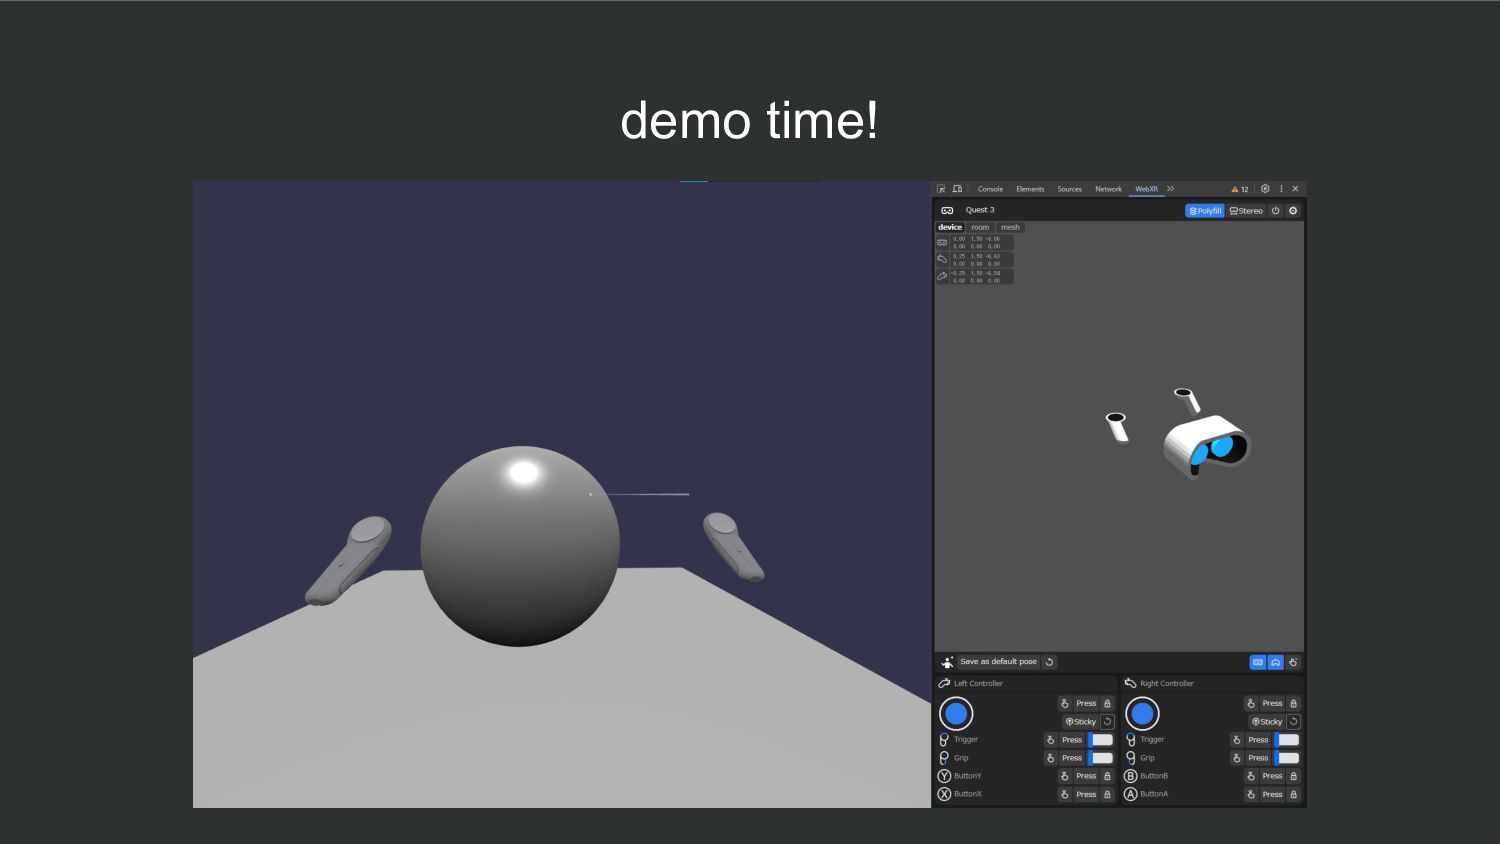
\includegraphics[width=0.8\textwidth]{stateXR.jpeg}
    \caption{Preview of XR context showing headset and controller interaction in Babylon.js}
\end{figure}
\newpage
\section{Materials and Methods}
\subsection{Tools and Technologies}

This project is built upon a combination of modern web and audio technologies that work together to provide a real-time, interactive 3D musical experience.

\paragraph{Babylon.js} is the primary 3D rendering engine used to construct the visual components of the application. It enables the creation of meshes such as spheres (balls) and boxes (obstacles), applies material textures and lighting, and manages the rendering loop. Babylon’s built-in Gizmo tools facilitate user interaction with the 3D objects—allowing for intuitive dragging, rotating, and resizing using mouse and keyboard inputs. The engine's picking system was used to implement selection logic for interactive obstacle manipulation.

\paragraph{Havok Physics} is integrated into Babylon.js and handles realistic simulation of forces and collisions. Each 3D mesh (ball or platform) is wrapped with a physics aggregate, enabling gravity, friction, and restitution effects. This provides lifelike physical behavior—balls bounce off platforms, react to gravity, and maintain momentum—all essential for generating sound through collision events. Havok’s rigid body system ensures accurate spatial interactions across frames.

\paragraph{WAM Pro-54 Synthesizer} is used to generate sound based on object collisions. WAM (Web Audio Modules) is a modern framework for browser-based audio synthesis. The Pro-54 emulates a classic analog synth, and in this project, it is triggered through MIDI messages when a sphere collides with a platform. A custom arpeggiator built into the system sequences notes according to predefined musical scales, providing musically coherent feedback rather than random sounds.

\paragraph{JavaScript and HTML5} form the backbone of the application logic. JavaScript manages the entire program flow, from setting up Babylon.js scenes and Havok physics to handling keyboard/mouse events, updating object states, and connecting to the audio system. HTML5 serves as the structural container via the `<canvas>` element for rendering the 3D scene.

Together, these technologies allow the simulation to be run entirely in a browser with no installation, making it highly accessible while showcasing modern web development capabilities.
\end{itemize}


\newpage
\subsection{Musical Logic: The Arpeggiator System}

At the heart of the audio generation process lies the arpeggiator, a system responsible for sequencing musical notes in a structured way. Instead of playing random notes, the arpeggiator ensures that each triggered sound adheres to a musically coherent pattern, enhancing the overall harmony of the system.

When the application starts, a musical scale is selected — for example, a C major scale. This scale is then converted into MIDI values using the \texttt{scaleToMidi} function. The MIDI note list is passed into the arpeggiator, which applies one of several patterns:
\begin{itemize}
    \item \textbf{Forward}: Plays the notes from start to end.
    \item \textbf{Backward}: Plays them in reverse order.
    \item \textbf{Alternate}: Moves up and down through the notes.
    \item \textbf{Random}: Randomly selects a note from the scale.
\end{itemize}
\begin{figure}[h!]
    \centering
    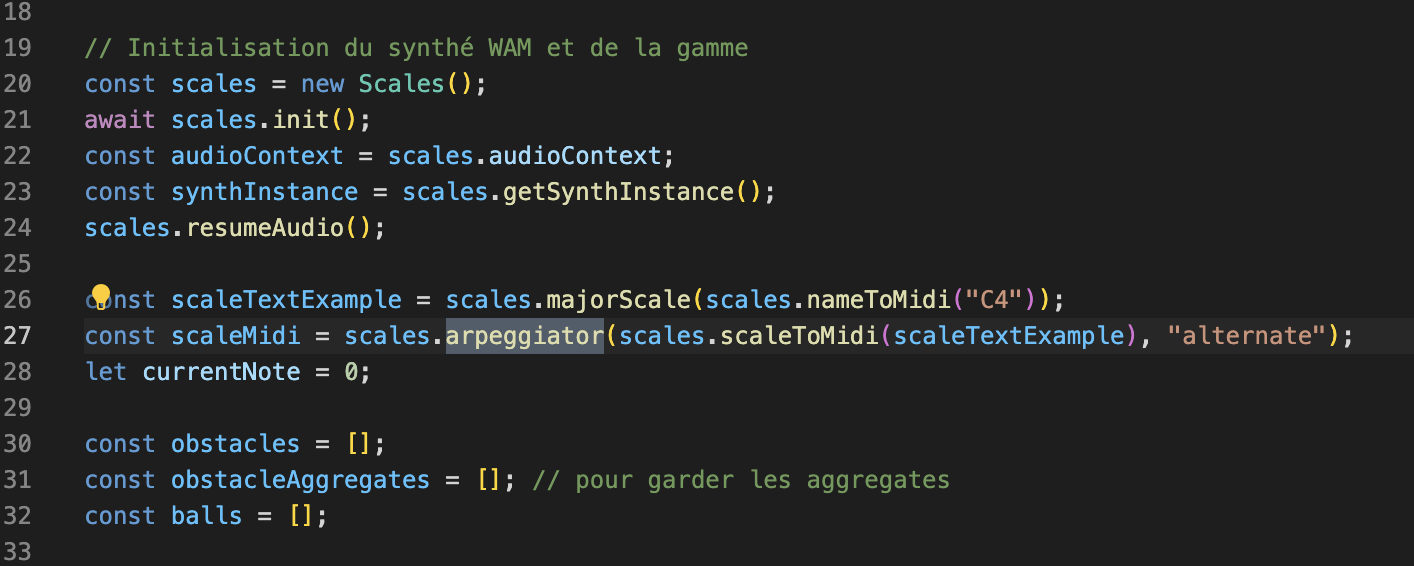
\includegraphics[width=0.8\textwidth]{arpeggiator.png}
    \caption{Visualization of the arpeggiator logic linking physics-based collisions to structured musical output.}
\end{figure}
Each collision with an obstacle triggers a MIDI note from this pattern. The arpeggiator keeps track of the current index and loops cyclically. This way, the sequence remains musically engaging without repeating the same note or pattern continuously.

Musically, this mimics how real synthesizers or DAWs operate when sequencing melodies, allowing users to perceive structure and progression even in a generative environment. This blend of deterministic logic and interactive physics is a key innovation in this project.
\subsection{Project Architecture and Logic}
The implementation began by linking the visual (Babylon) and physics (Havok) layers. Every obstacle is instantiated with a physics aggregate to track its physical interactions. Once placed, they can be rotated or resized using Shift/Ctrl keys and mouse dragging. The position, rotation, and physics body are updated synchronously.

Upon each mouse click (outside of a drag operation), a new ball is instantiated. The physics engine calculates its fall and collision response. A collision event with an obstacle triggers a MIDI note via the WAM Pro-54 synth. The notes follow an arpeggiated scale generated at startup.

The \texttt{scales.js} file abstracts music theory. It includes functions for scale generation (major, minor, blues, pentatonic, etc.), conversion of MIDI values to note names, and applying transformations like forward, backward, or randomized arpeggiation.

The logic combines visual design, physics realism, and audio sequencing into a minimal but powerful system for interactive sound synthesis.

\begin{figure}[h!]
    \centering
    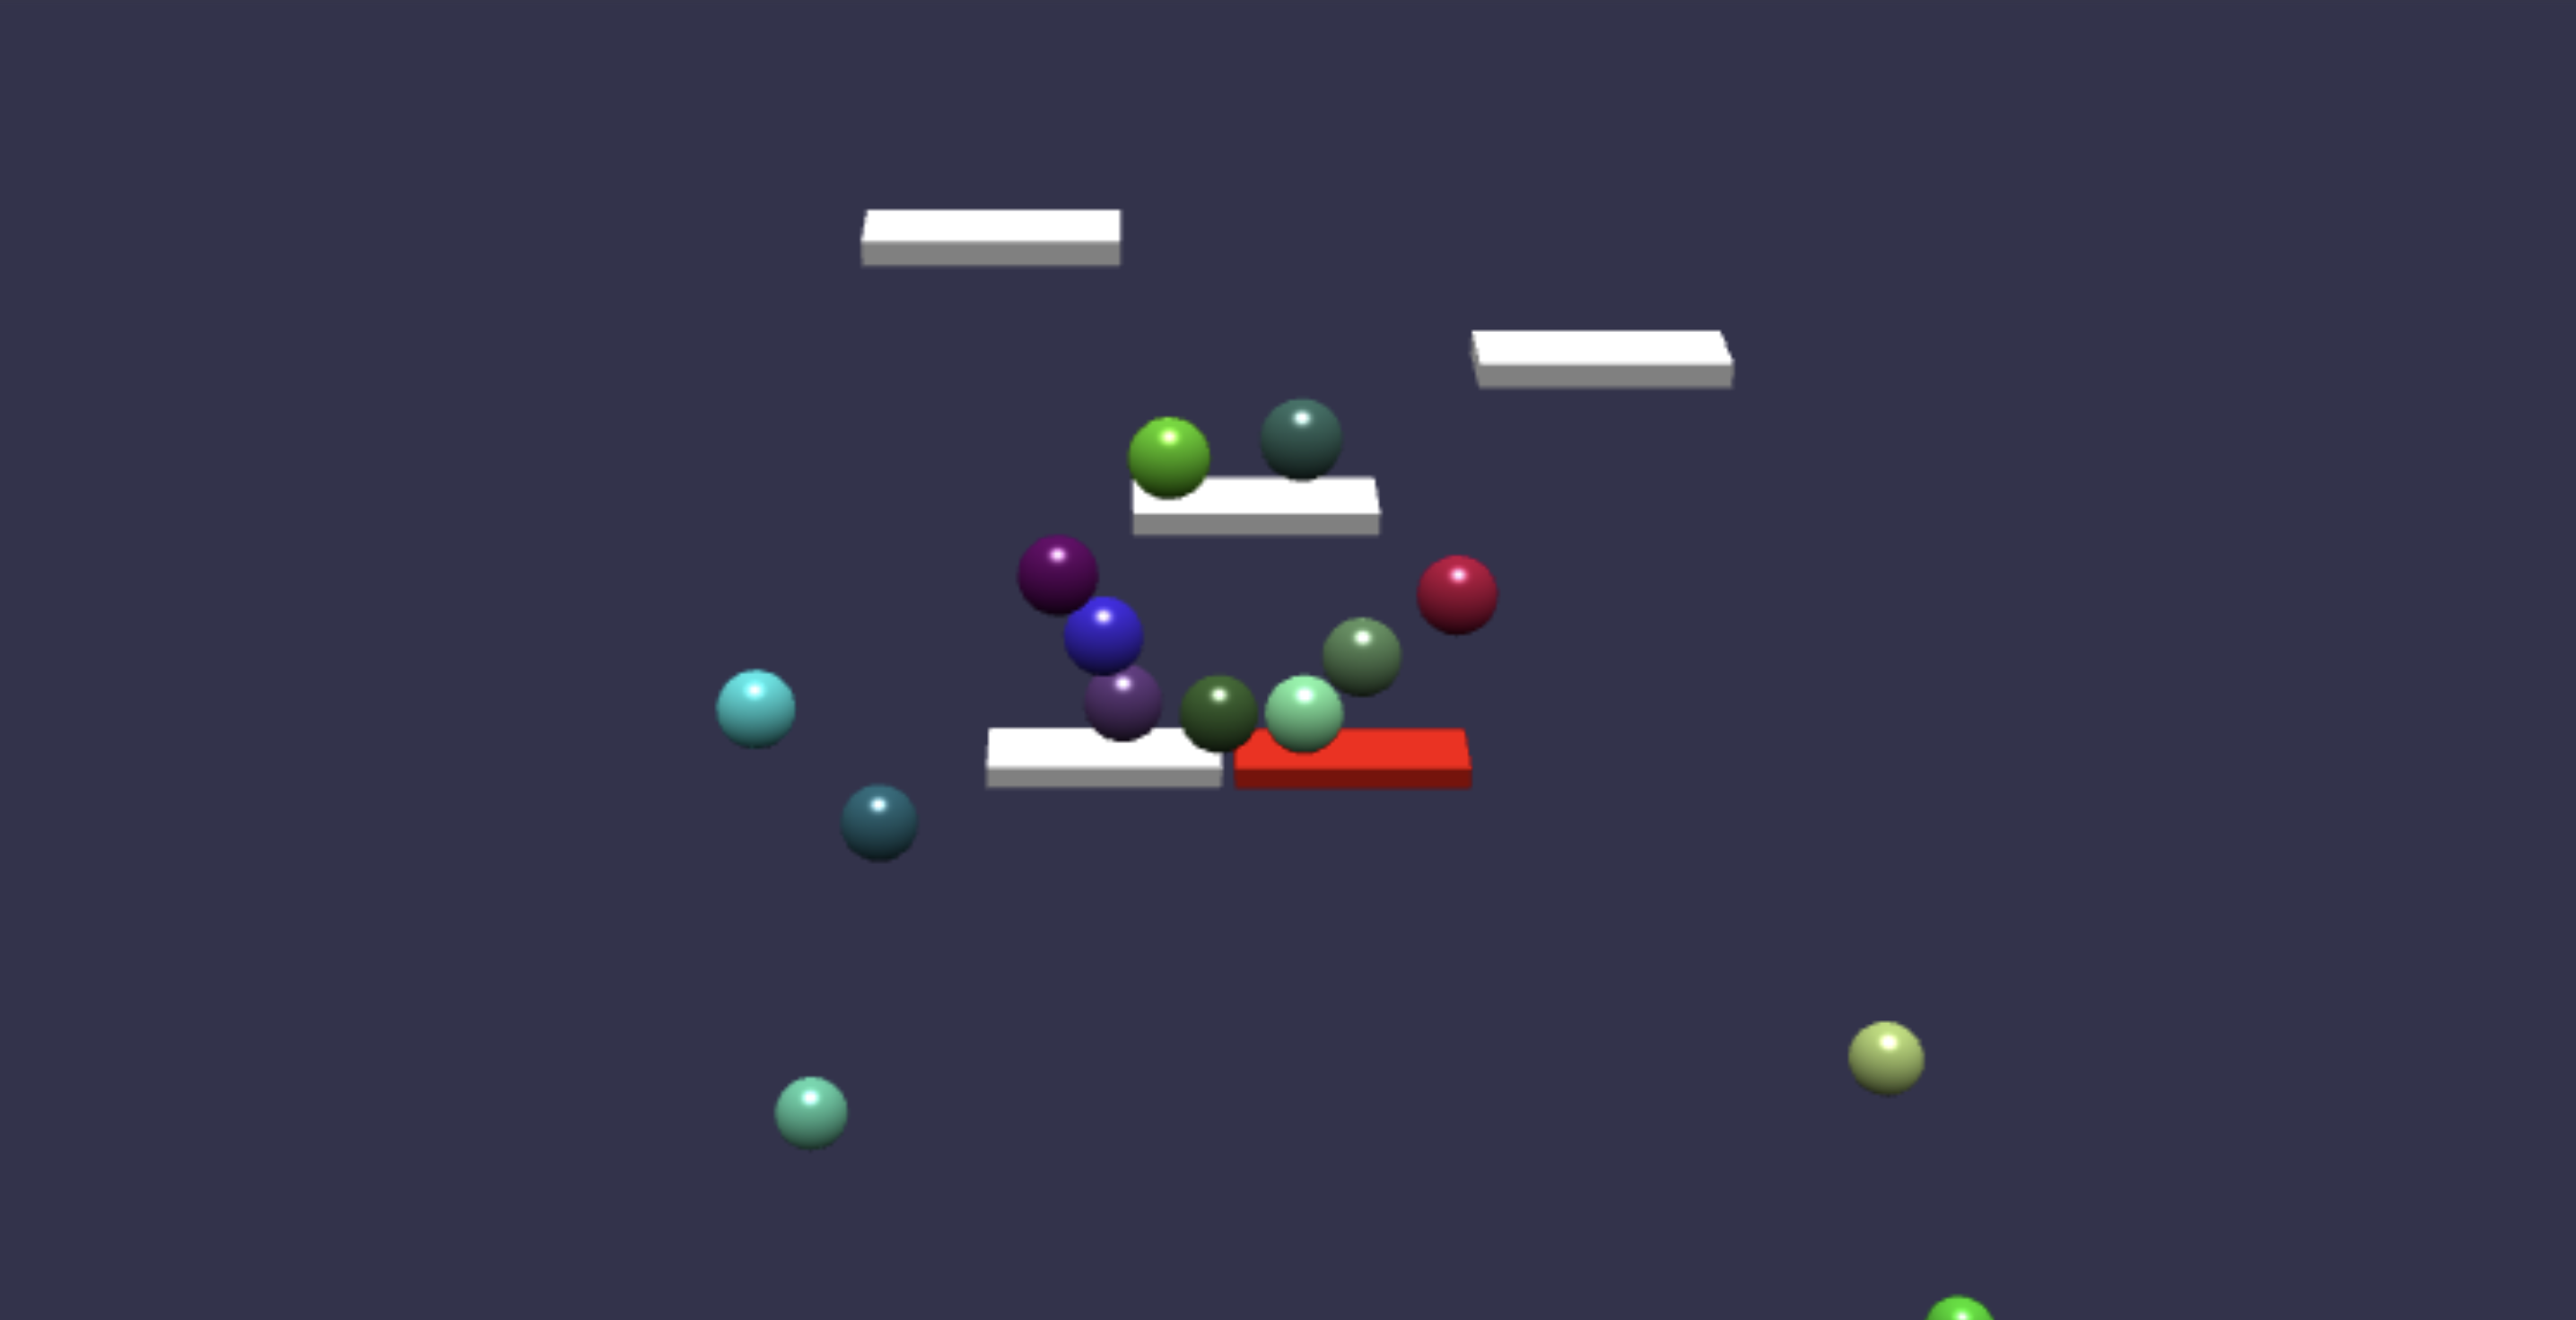
\includegraphics[width=0.8\textwidth]{coloredSpheres.png}
    \caption{Scene with interactive spheres bouncing on obstacles, triggering musical notes.}
\end{figure}

\begin{figure}[h!]
    \centering
    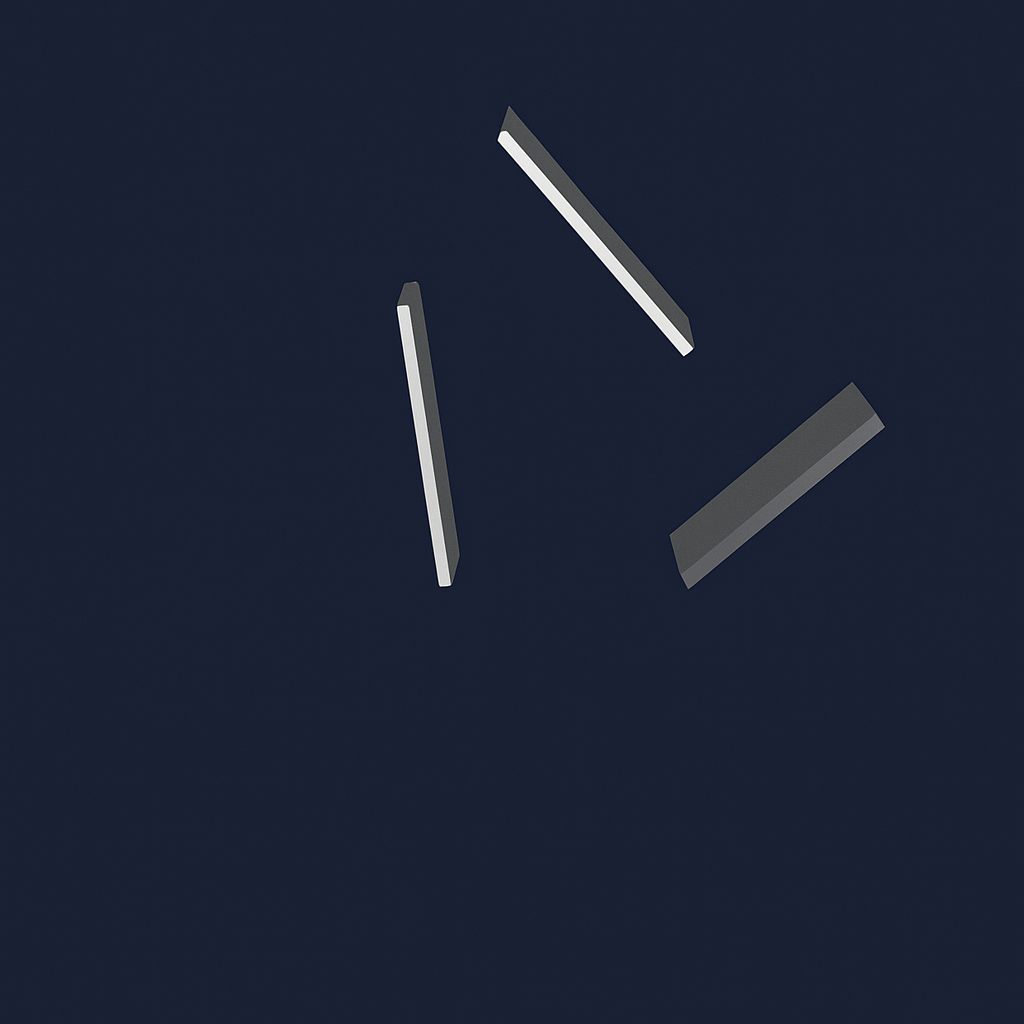
\includegraphics[width=0.8\textwidth]{rotated.png}
    \caption{Obstacles in distinct rotations demonstrating Gizmo interaction.}
\end{figure}

\begin{figure}[h!]
    \centering
    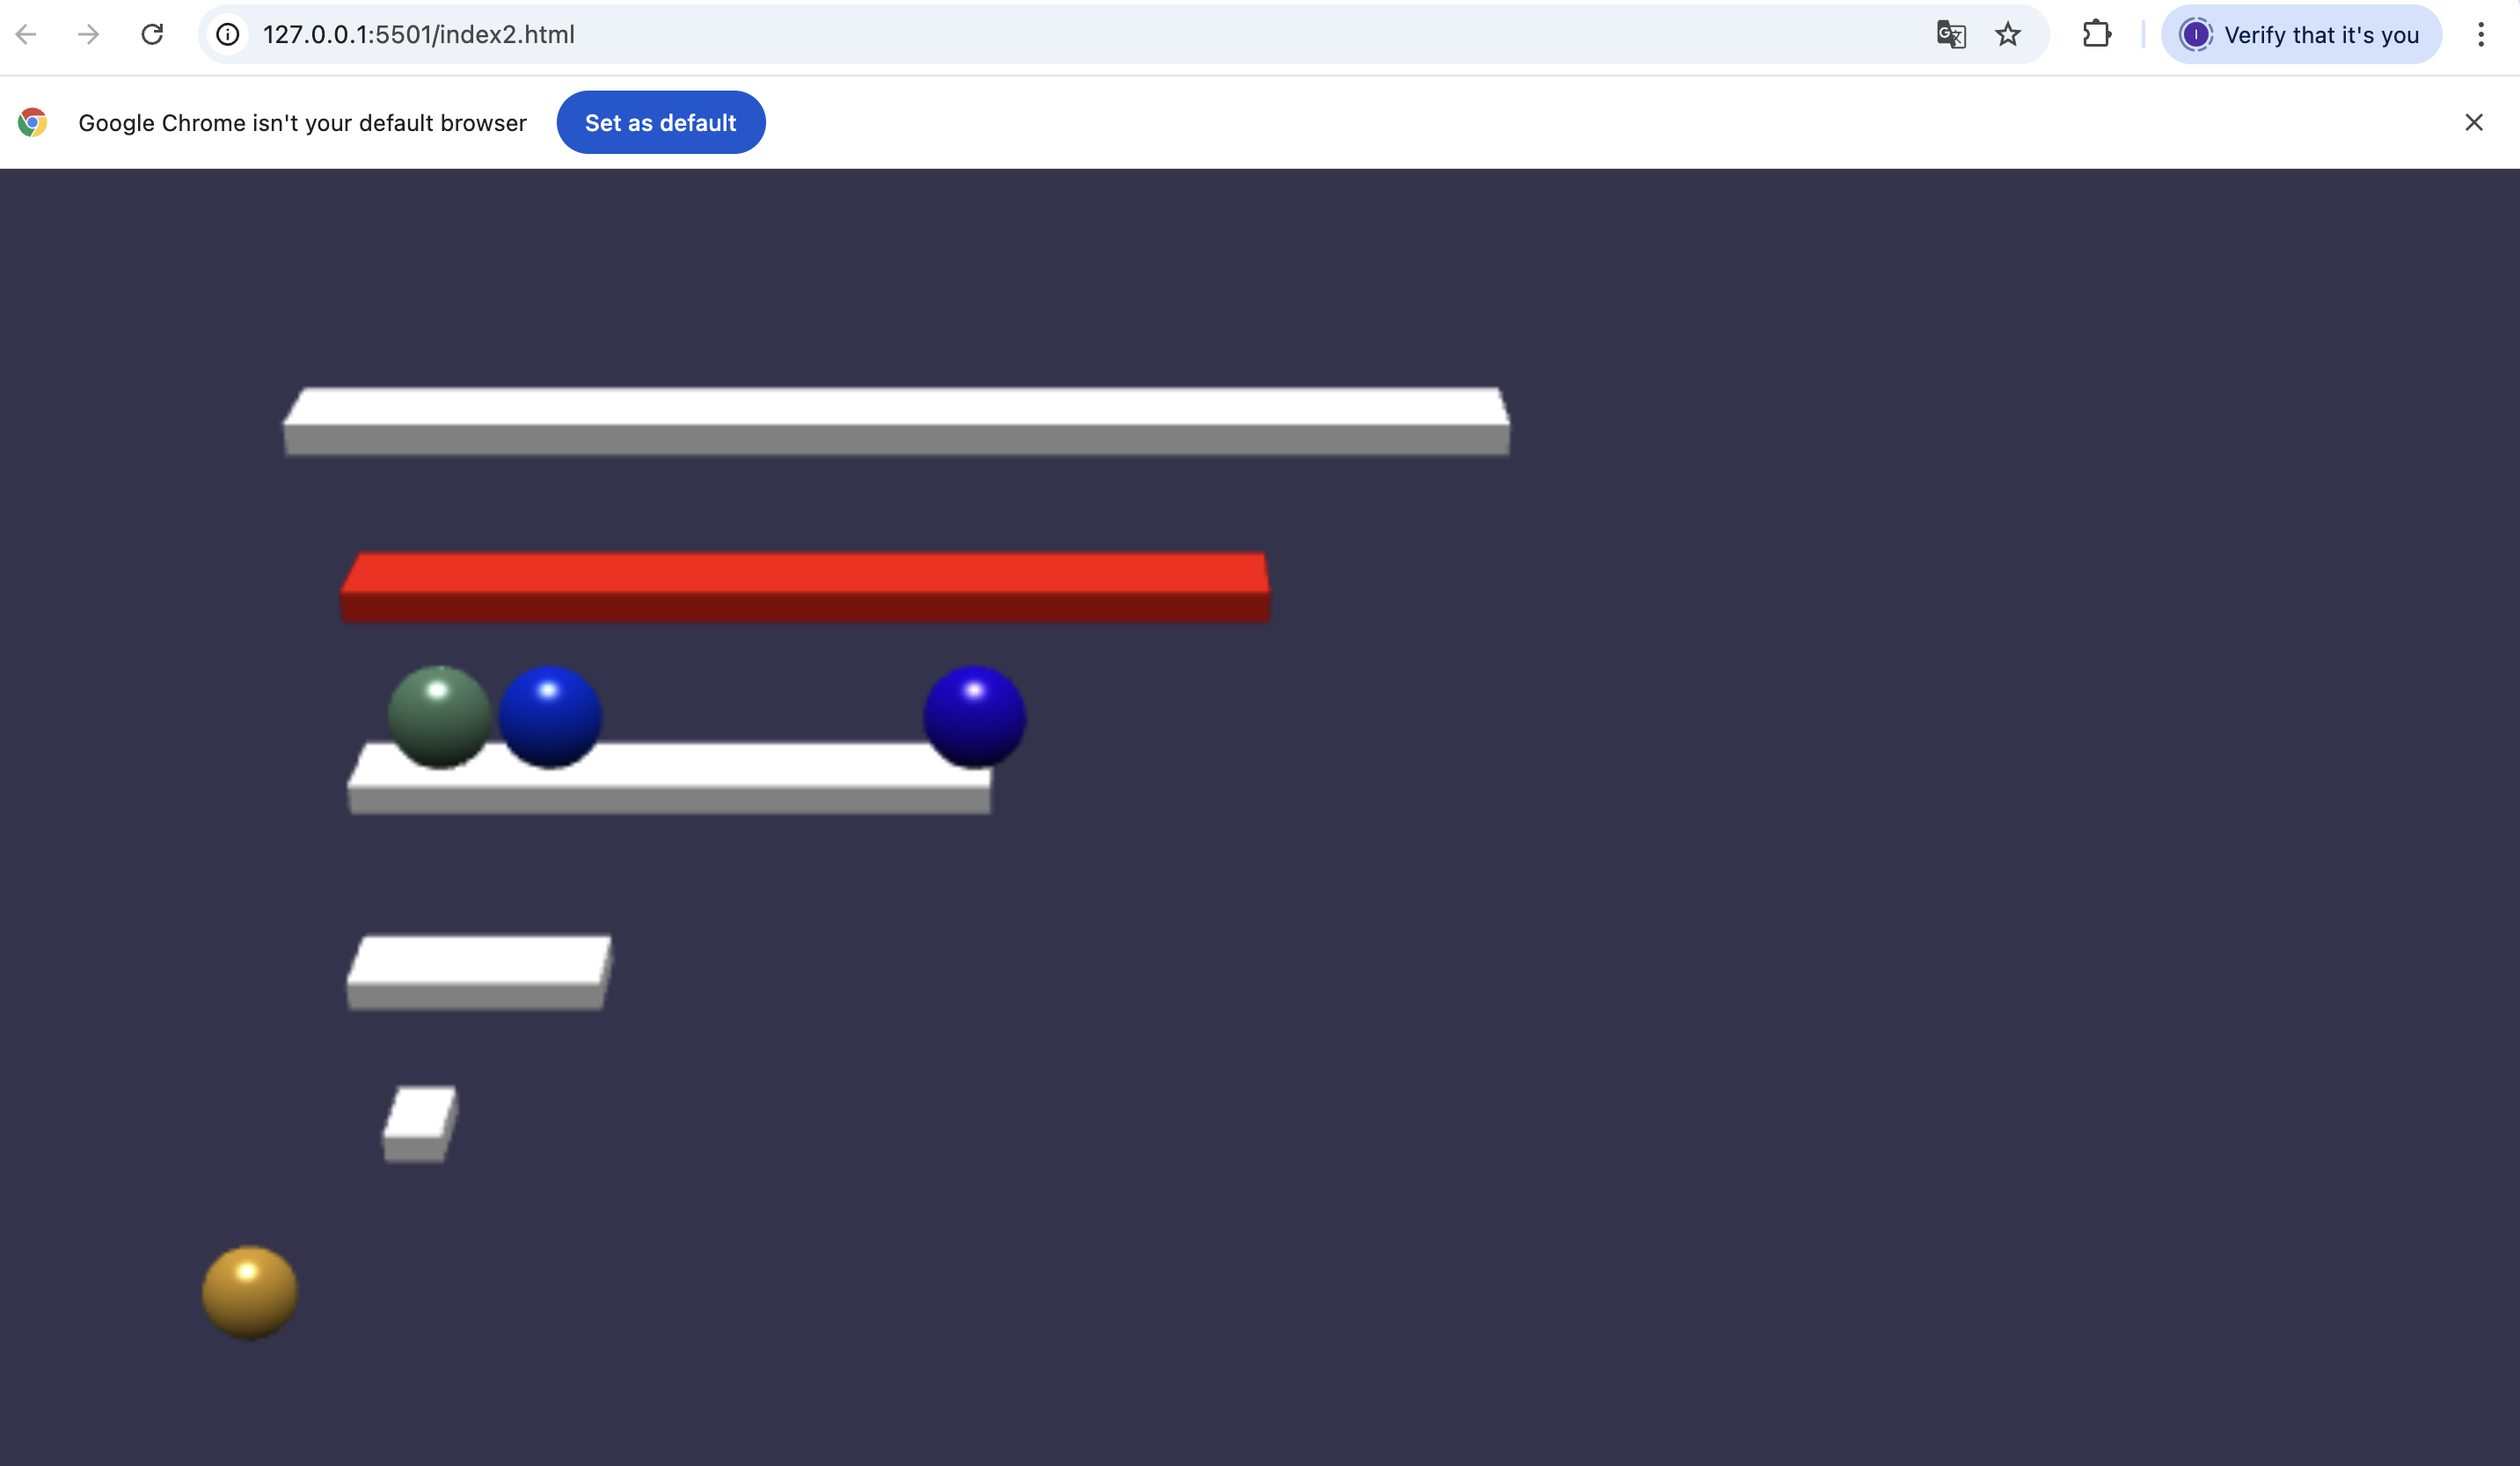
\includegraphics[width=0.8\textwidth]{sizingobstacles.png}
    \caption{Scaling obstacles with Ctrl + mouse drag.}
\end{figure}
\newpage
\section{Results}
\subsection{Interaction Quality}
The final application provides a smooth, responsive, and immersive user experience. Users are presented with a 3D scene containing platforms and falling spheres. The user can:
\begin{itemize}
    \item Add new platforms using the \texttt{N} key.
    \item Select and move them with mouse drag.
    \item Resize using Ctrl + drag, or rotate using Shift + drag.
    \item Drop a new sphere with a simple click.
\end{itemize}

\subsection{Audio Feedback}
Each collision with a platform triggers a MIDI note. The sound feedback aligns precisely with the visual event, creating a harmonized experience. Different arpeggiation patterns allow for variety in musical output.
\newpage
\section{Discussion}

\subsection{Strengths}
One of the main strengths of this project lies in its real-time interaction capabilities. Users can actively engage with the scene by generating spheres, modifying obstacles, and triggering sounds upon collision, all in a seamless, responsive environment. This immediate feedback loop creates a strong sense of presence and immersion, essential for an engaging interactive musical experience.

Another significant advantage is its web-based implementation. The application is accessible via a standard web browser, requiring no installation or setup, making it widely available across platforms. This enhances usability and encourages broader experimentation and engagement.

Furthermore, the system's architecture is modular. The separation of concerns between physics (Babylon.js + Havok), audio (WAM + Web Audio API), and visual interaction (Gizmos, input events) provides flexibility and scalability. Future developers can extend or adapt components—such as the synthesizer, scale generator, or collision handling—without disrupting the core functionality.

Finally, the immersive combination of 3D visuals and harmonic sound synthesis strengthens user engagement. The user doesn't just observe the environment—they actively shape it, visually and sonically. This dual feedback (audio and visual) adds depth to the overall interaction.

\subsection{Limitations}
Despite the promising results, the project faced several limitations. First, manipulating obstacles (rotating or resizing) required manually updating their associated physics aggregates. This process is error-prone and non-intuitive, especially for real-time usage. A smoother integration between object transformation and physics synchronization would greatly enhance usability.

Another challenge stemmed from the camera control configuration. In order to enable intuitive object manipulation (rotation via Shift, scaling via Ctrl), the default camera interactions had to be disabled or constrained. This created tradeoffs in the user experience, limiting fluid navigation when editing the scene.

Additionally, precise interaction using Gizmos was sometimes inconsistent, particularly in edge cases where objects overlapped or when attempting fine-grained adjustments. Improved UX handling or snap-to-grid features could alleviate such issues.

Finally, the system currently lacks persistent state or export options. Once the page is refreshed, all configuration is lost. This limits long-term creativity or reproducibility of complex musical arrangements.

\subsection{Future Improvements}
Looking ahead, several avenues for improvement could enhance both the system's usability and functionality. The most immediate enhancement would be a comprehensive user interface, including sliders and controls for object properties like mass, bounce, friction, and pitch mapping. This would empower users to customize the environment without interacting directly with the code or relying solely on keyboard shortcuts.

Another key feature would be the ability to export generated melodies or sequences in standard formats such as MIDI. This would make the system not only interactive but also productive—allowing artists or researchers to repurpose the musical output in other software or contexts.

Furthermore, integration with WebXR would unlock collaborative and immersive potential. Users equipped with VR headsets could enter the shared scene, interact with objects, and co-create soundscapes together. This would align the project with the broader goals of the Musical Metaverse initiative and facilitate new forms of distributed musical collaboration.
\newpage
\section{Conclusion}
This project successfully combines physics simulation, real-time sound synthesis, and intuitive user interaction to create a compelling, browser-based musical playground. It demonstrates the feasibility of linking physical behavior with musical events using open web standards and modular architecture. 

Beyond technical implementation, it contributes a unique interaction model—where collision, scale, and position inform sound output, giving users tangible control over harmony and rhythm. It also highlights both the creative power and the challenges of building such systems, particularly in synchronizing physics engines with audio frameworks.

As a proof-of-concept, the system provides a strong foundation for future work. With additional features like export, UI, and XR compatibility, it could evolve into a fully-fledged tool for digital musicians, educators, or VR artists exploring the boundaries of sound, space, and interactivity on the web.


\newpage
\section*{References}
\begin{itemize}
    \item Buffa, M. \textit{Internet of Sounds 2024 – Web Audio Modules in the Musical Metaverse.}
    \item Babylon.js Documentation. \url{https://doc.babylonjs.com/}
    \item Web Audio Modules SDK. \url{https://webaudiomodules.org/}
    \item Havok Physics integration in Babylon.js. \url{https://www.babylonjs.com/havok/}
    \item Mozilla Web Audio API documentation. \url{https://developer.mozilla.org/en-US/docs/Web/API/Web_Audio_API}
    \item A. Kapur et al. \textit{A Framework for Mapping Physical Motion to Musical Expression} (2005)
\end{itemize}

\end{document}
